\section{Data Acquisition}

%head
The following section will include a description on how the data for the study have been acquired and processed. All data processing, along with GUI design and implementation, will be done in Matlab.

%presentaion of training GUI
To acquire data a training GUI has been designed and implemented in Matlab. The GUI has been designed to fulfil the specific needs for this project. An illustration of the GUI can be seen in \figref{fig:GUI_Training}. 

\begin{figure}[H]
	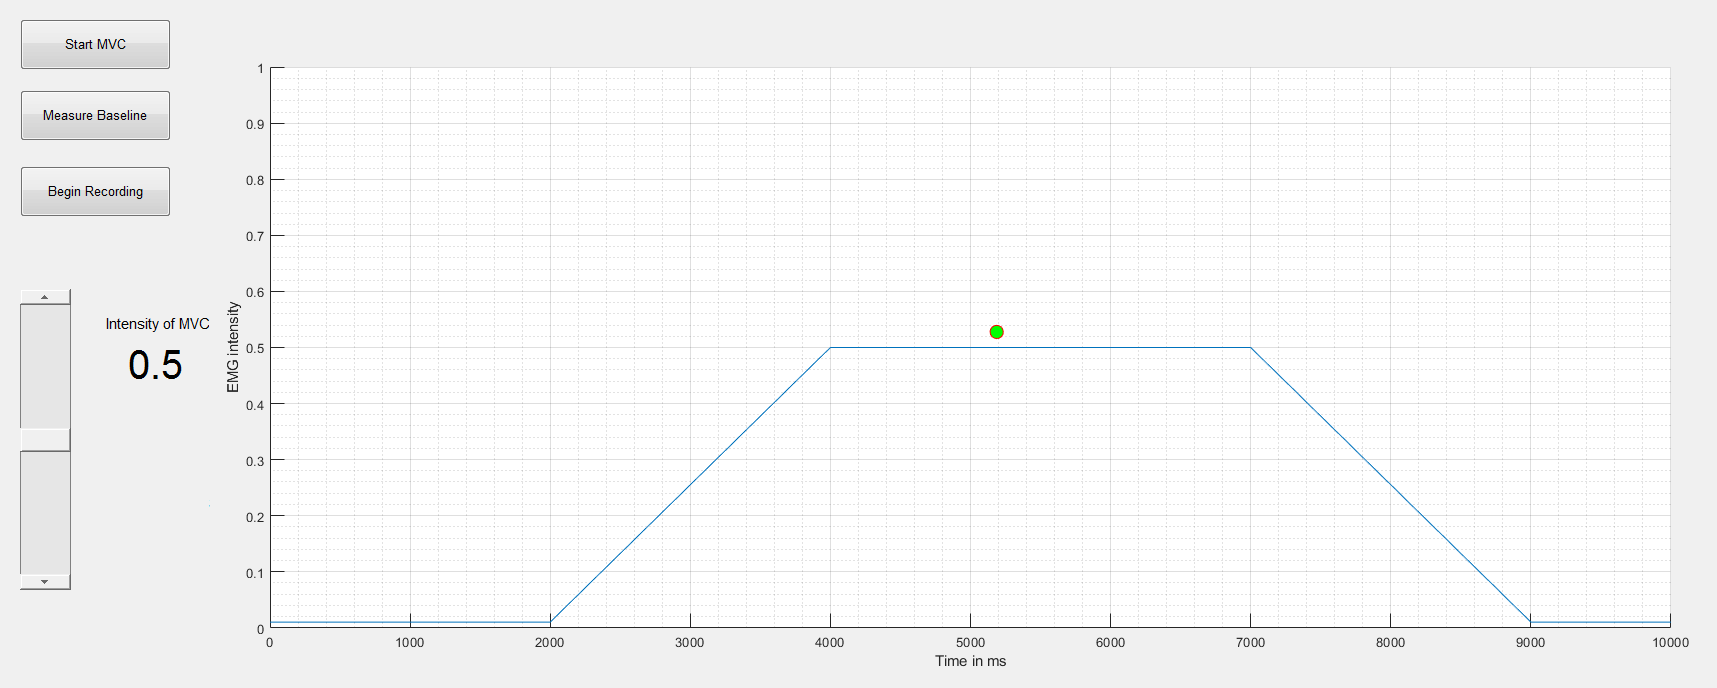
\includegraphics[width=.9\textwidth]{figures/GUI/GUI_Training.png}
	\caption{The training GUI implemented with Matlab GUI development environment. Control buttons to calculate MVC and perform MVC fraction recordings are placed on the left side. The trapezoid plot with the green dot controlled by the input EMG signal from the subject is shown on the right. The fraction of the MVC can be defined by the slider located under the control buttons.}
	\label{fig:GUI_Training}
\end{figure} 


%%%%%%%%%%%%%%%%%%%%%%%%%%%%%% moved from its own section %%%%%%%%%%%%%%%%%%%%%%%%%
%\textbf{maybe not needed now (Motor unit action potential (MUAP) can be easily decribed as the addition of the action potentials emerging from the muscle fibers comprising the motor unit. The EMG signal is the result of the inclusion of different MUAP.)}
%
%%This depends on the task. It is true if you do the ramp-and-hold contractions like you do, but you cannot divide all contractions into two states. So this is something that is mostly related to your training protocol. 
%%the steady and transient is related to the contraction profile (trapezoid) that is used to record training data. As Jakob said, this is specific to prosthesis control and should be therefore moved to a different section. In addition, this is not the only profile that is being used (some use ramp profile for example, from min to max, where there is no steady state).
%\textbf{Jakob/Strahinja Coments:For this study, the EMG data acquisition was depicted through a trapeze. The subjects had to follow the shape of the trapeze while performing the desired wrist movement. To facilitate the task a green dot was shown, which moves with time in relation to the normalized intensity. The training protocol was done in such a way that was possible to differentiate between two states of the EMG signal.} 
%
%The transient state, related to the beginning phase of the muscle contraction and the steady state which is the stable phase of the muscle contraction when a constant position is held. \cite{mobarak2014}
%
%Although the steady state only contains a short temporal structure of the patterns involved in the contraction of the muscle \cite{mobarak}, studies has shown that it is possible to achieve online continuous control using steady-state EMG signals. A study by Englehart et al. \cite{englehart} demonstrated that steady-state data classified more precisely than transient state data. This could be due to the fact that a larger amount of meaningful data is contained in this muscle contraction phase \cite{mobarak}. For the training of the control system in this project the steady signal will then be used. %However there are still limitations due the fact that the classifier can not deal with the transient EMG signals. Some clinical applications that combine both data have shown an increase in the recognition system. 
%%%%%%%%%%%%%%%%%%%%%%%%%%%%%% moved from its own section %%%%%%%%%%%%%%%%%%%%%%%%%

The functions of the GUI consists of a baseline measurement button, a MVC measurement button, a data recording button and a fraction of MVC intensity slider. The baseline measurement is acquired for the purpose of being subtracted from the signal, in order to remove the signal artefacts that are present. At the baseline acquisition the subject is resting the lower arm in the given limb position. The MVC is calculated as a mean of the maximum values in each of the eight channels, and is set as a normalized reference point of 1. The MVC is a contraction at the intensity of which the subject can withhold for 15 seconds. The data recording contains the raw data of a given fraction of the MVC. The fraction is decided by setting the slider to the wanted fraction value, before the recording is started. The slider sets the fraction value so the plateau of the trapeze is at the set value. The trapeze depicts an initial resting phase of two seconds with the intensity of 0, a transition phase of two seconds with an ascending slope until the plateau phase is reached, which has a three second duration, and then a final descending transition phase of two seconds and resting phase of one second. 
For the project only data acquired from the steady state of the signal, meaning the plateau of the trapeze, will be used in data processing. Although the steady state only contains a short temporal structure of the patterns involved in the contraction of the muscle \cite{mobarak}, studies has shown that it is possible to achieve online continuous control using steady-state EMG signals. A study by Englehart et al. \cite{englehart} demonstrated that steady-state data classified more precisely than transient state data. This could be due to the fact that a larger amount of meaningful data is contained in this muscle contraction phase \cite{mobarak}.

Data acquisition will begin by recording of the baseline in the limb position and the MVC of the movement to be tested. Initialization of the recording will show a green dot, which moves with time in relation to the normalized intensity. The green dot is calculated as the mean of the input EMG signal in a 200 ms window with a 100 ms overlap. Meanwhile IMU data for the orientation of the arm is being recorded and saved for later use. %The signal is afterwards normalized with the MVC measurement as the reference point. 
From this acquired data features will be extracted and used to train regressors for each of the subjects for each of the hand gestures performed.


